\section{Annex}

\subsection{Figures}
\begin{table}[h]
\centering
\caption{DWG / DXF evaluation matrix.}
\label{tbl:DWGEvaluationMatrix}
\begin{tabular}{@{}llllllll@{}}
\toprule
Name         & Vendor         & Price        & Last Update      & License           & Read & Write & Comment                             \\ \midrule
YCAD Library & Ed Karlo       & -            & August 07, 2015  & LGPLv2            & Yes  & ?     & Very confusing \& no documentation. \\
Teigha       & ODA            & 2000 USD / Y &                  & Commercial        & Yes  & Yes   &                                     \\
Kabeja       &                & -            & March 12, 2008   & Apache License v2 & Yes  & No    &                                     \\
Tika         & Apache         & -            & October 19, 2016 & Apache License v2 & Yes* & No    & *Meta text reader.                  \\
jnetcad      & Johannes Raida & ?            & April 28, 2016   & Commercial        & Yes* & Yes*  & *Only converter for 3D Objects.     \\
CaffViewer   & DeCaff         & 1350 Euro    & May 17, 2016     & Freeware          & Yes  & Yes   &                                     \\ \bottomrule
\end{tabular}
\end{table}

\pagebreak
\subsection{Developer Guide}
This section describes, how to extend the application developed in this work. It is split into different tasks, which will most likely be done in the future.

\subsubsection{Adding new algorithm}
To add a new algorithm you have to create a new class, which implements the \textit{IAlgorithm} interface. The interface and algorithms are described in section~\ref{sub:algorithm}, but we will give you here a short overview over the interface and how to implement it.

We recommend, to split up different parts of a new process into different algorithms, which enhances the maintainability of an algorithm.

\begin{figure}[h]
  \centering
      \includegraphics[width=0.6\textwidth]{IAlgorithm_CD}
  \caption{Algorithm interface class diagram.}
  \label{fig:IAlgorithm_CD_DG}
\end{figure}

In figure~\ref{fig:IAlgorithm_CD_DG} you see the methods, which have to be implemented to run the algorithm. The very basic version of an algorithm just returns the input image as it is (Listing \ref{lst:basicAlgorithm}).

\begin{lstlisting}[caption={Basic version of an algorithm.}, label={lst:basicAlgorithm}, language=Kotlin]
class MyAlgorithm : IAlgorithm
{
    override val name: String
        get() = "MyAlgorithm"

    override fun run(image: AFImage, history: MutableList<AFImage>): AFImage {
        return image
    }
}
\end{lstlisting}

If you change the original image, it makes sense to create a copy of the incoming image, because the algorithm will maybe run multiple times. There are multiple ways to copy a \textit{Mat}, but we have provided an extension method called \textit{copy()} (Listing~\ref{lst:extendedAlgorithm}, Line~\ref{line:AlgorithmCopy}), which creates a deep copy of the image.

If your algorithm uses parameters, which should be possible to change by the user, you can flag the parameter variables with an \textit{AlgorithmParameter} attribute (Listing~\ref{lst:extendedAlgorithm}, Line~\ref{line:AlgorithmParameter}). You then also have the possibility to set the range of the parameter and provide a short help text (Listing~\ref{lst:extendedAlgorithm}, Line~\ref{line:AlgorithmHelpText}). These informations will be read by the parameter window and shown during the process.

\begin{lstlisting}[caption={Extended version of an algorithm.}, label={lst:extendedAlgorithm}, language=Kotlin, escapechar=$]
class MyAlgorithm : IAlgorithm
{
    @AlgorithmParameter(name = "Threshold",
            minValue = 0.0,
            maxValue = 255.0,
            majorTick = 1.0,
            helpText = "Set the threshold value!") $\label{line:AlgorithmHelpText}$
    var threshold = 128.0 $\label{line:AlgorithmParameter}$

    override val name: String
        get() = "MyAlgorithm"

    override fun run(image: AFImage, history: MutableList<AFImage>): AFImage {
        val img = image.image.copy() $\label{line:AlgorithmCopy}$
        
        // do image processing
        img.threshold(threshold)

        history.add(AFImage(image.image, "Image before threshold")) $\label{line:AlgorithmHistory}$
        return AFImage(img, "Result")
    }
}
\end{lstlisting}

To provide images to the user from between the algorithm, you just have to add the image to the \textit{history} list (Listing~\ref{lst:extendedAlgorithm}, Line~\ref{line:AlgorithmHistory}). The images provided in there are shown in the parameter window (Section~\ref{sub:parameter_window}).

\subsubsection{Extending the user interface}

To edit the user interface, you have to edit the \textit{MainWindow} controller class. In this section we will explain how to add a new button to the user interface, to export the current displayed image.

The user interface is written with the UI Framework JavaFX 2 and uses FXML files to define the layout of the different forms. We recommend to use the \todo{add link}SceneManager application from Oracle to edit these layout files.

For more information about the user interface, have a look at the section~\ref{sub:userInterface}.

\begin{figure}[H]
	\centering
	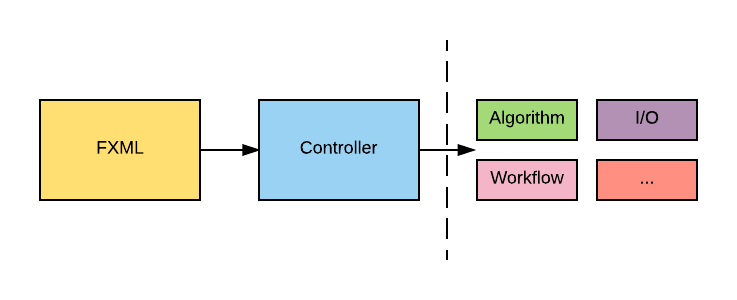
\includegraphics[width=0.8\textwidth]{fxmlArchitecture}
	\caption{User interface architecture.}
	\label{fig:fxmlArchitecture}
\end{figure}

As seen on figure~\ref{fig:fxmlArchitecture}, the user interface is split into two parts. The first one is called FXML and defines the layout of the interface. The second one is the controller, which defines the actions and events, which can happen on the interface. For example, for the \textit{MainWindow} there is a \textit{MainWindow.fxml} and a \textit{MainWindow.kt} file in the source code.

\begin{lstlisting}[caption={MainWindow.fxml with new button.}, label={lst:fxmlwithbutton}, language=XML, escapechar=$]
    <Separator orientation="VERTICAL" />
    <Button onAction="#exportLayer" text="Export SVG" />
    <Button onAction="#exportToCSV" text="Export CSV" />
    <Button onAction="#saveImage" text="Save Image" /> $\label{line:fxmlSaveImage}$
</children>
\end{lstlisting}

First of all, you have to add the extra button to the layout. In listing~\ref{lst:fxmlwithbutton} on line~\ref{line:fxmlSaveImage} there is the new button defined. The \textit{onAction} attribute is a link to a method in the controller of the view.

Now, you have to implement the behaviour of the button on the controller side. There you have to create a function, which is called like the \textit{onAction} attribute value.

\begin{lstlisting}[caption={Save image controller code.}, label={lst:saveImage}, language=Kotlin, escapechar=$]
fun saveImage(e : ActionEvent)
{
    val stage = (e.source as Node).scene.window as Stage

    val fileChooser = FileChooser()
    fileChooser.initialFileName = "image.png"
    fileChooser.title = "Export image as png"
    fileChooser.extensionFilters.addAll(
            FileChooser.ExtensionFilter("PNG", "*.png"))

    val file = fileChooser.showSaveDialog(stage)

    if (file != null) {
        val writableImage = WritableImage(canvas.canvas.width.toInt(),
                canvas.canvas.height.toInt())
        canvas.canvas.snapshot(null, writableImage)
        val renderedImage = SwingFXUtils.fromFXImage(writableImage, null)
        ImageIO.write(renderedImage, "png", file)
    }
}
\end{lstlisting}

First, you have to show a file chooser, where the user is able to choose the file output location. To save the current image, you have to copy the canvas element into a writable image.

\subsubsection{Training new classifiers}

The objection detection in this project is primarily achieved with cascade classifiers (Section~\ref{sub:CascadeTraining}). This section gives a brief overview, how to train new objects with cascading classifiers and how to add it to the current process.

To train a new object, you should have following prerequisites:

\renewcommand{\labelenumi}{\alph{enumi})}
\begin{enumerate}
    \item Minimum 25 images of the object to detect (positives).
    \item Minimum 50 large images of the background (negatives).
    \item OpenCV installed (http://opencv.org/).
    \item ImageMagick installed (https://www.imagemagick.org/).
    \item OpenCV Sample Annotator installed (https://github.com/cansik/opencv-sample-annotator).
\end{enumerate}

\paragraph{Setup new training project}

The source code of this project contains a folder called \textit{/training}, which contains a shell script called \textit{train.sh}. This shell script is there to train a new classifier, but it needs some files at the right place to run.

The folder also contains an example directory structure called \textit{/training/example}. We recommend to copy this structure, rename it to the object, you want to recognise (for example \textit{doors}) and add your positive images to the \textit{positive} folder and the negative images to the \textit{negative} folder.

\paragraph{Annotate positive images}

Now you have to annotate your positive files, which means that you have to select the object in your positive images. We have developed a simple application (Figure~\ref{fig:SampleAnnotator}), which helps you to annotate the images.

\begin{figure}[H]
	\centering
	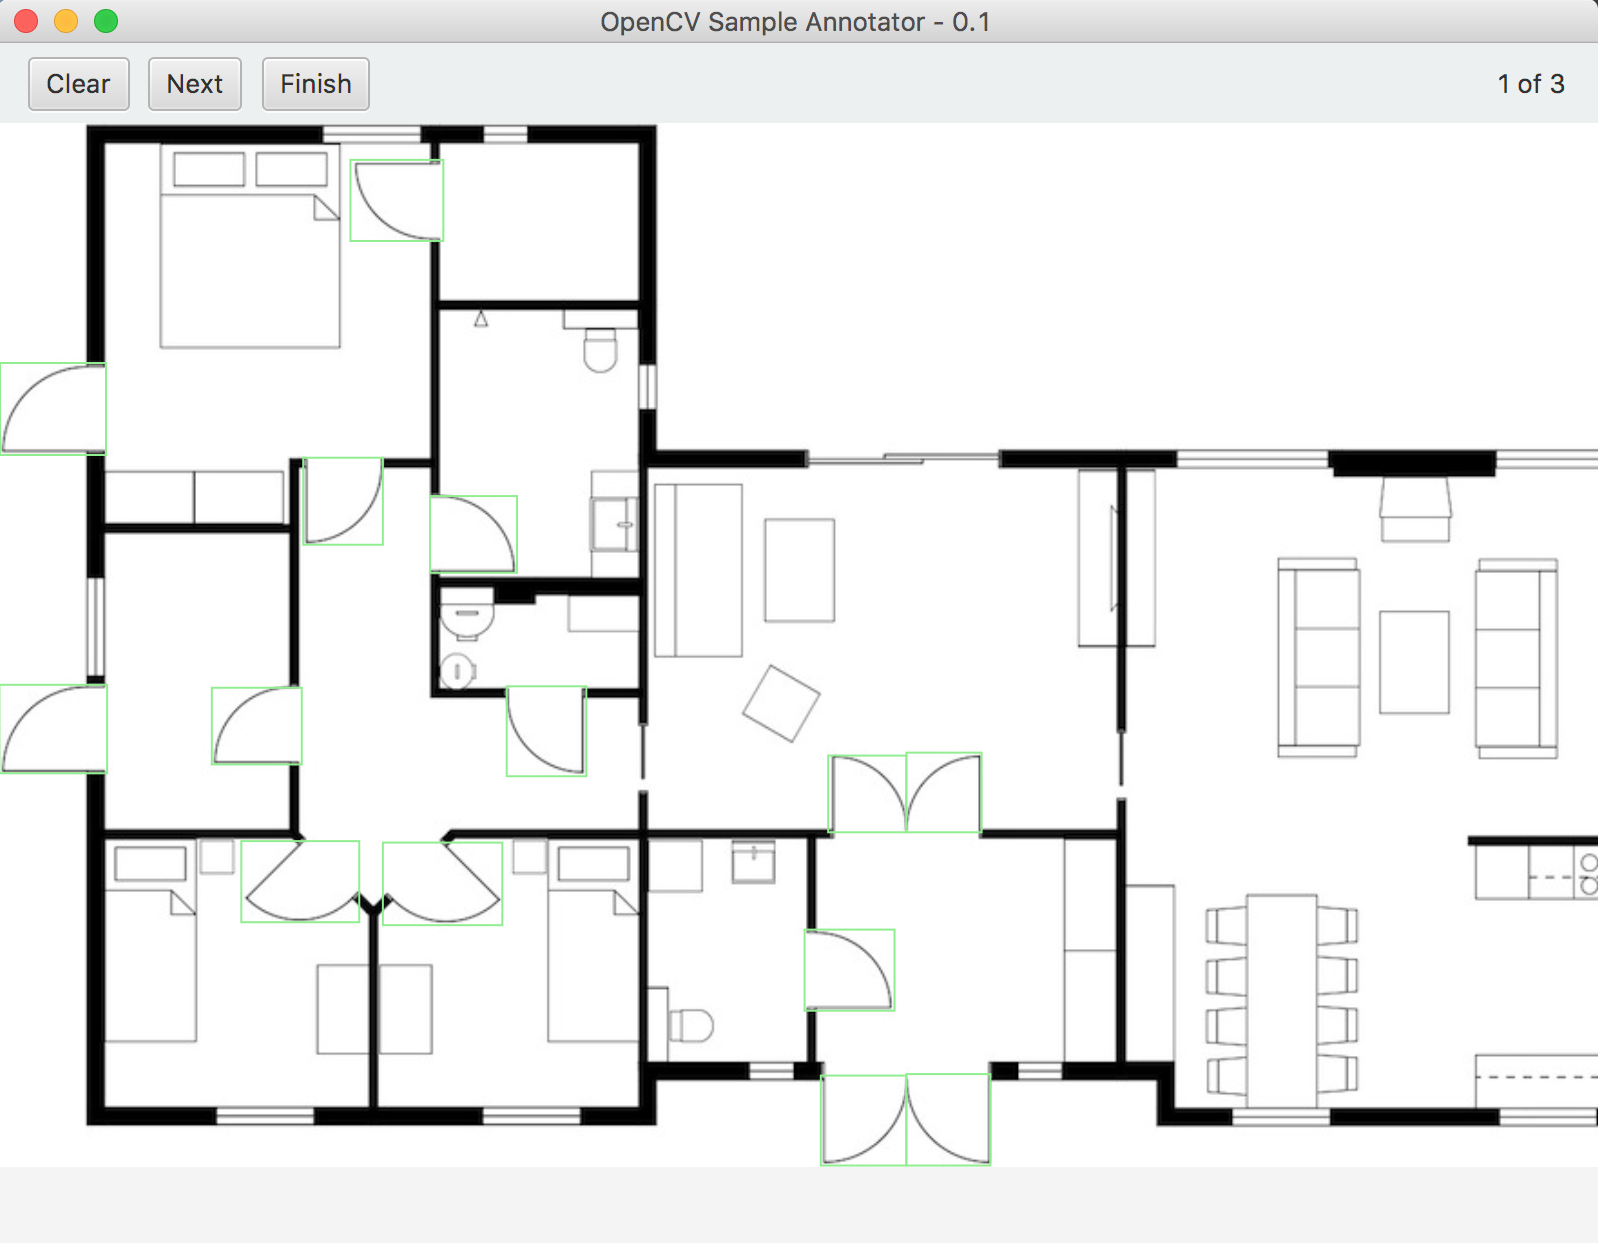
\includegraphics[width=0.8\textwidth]{SampleAnnotator}
	\caption{OpenCV Sample Annotator.}
	\label{fig:SampleAnnotator}
\end{figure}

If you start the application, you have to select the dataset. These are your positive images, which are stored in the \textit{positive} folder. The second thing to select, is the output file. You should store it directly into the project folder (\textit{/training/doors}) as \textit{positives.txt}.

Then you have to draw a rectangle around every object, that occurs in the image. If you have annotated all objects, click next and annotate the next image until you are finished. The application automatically saves the annotated regions into the \textit{positives.txt} file.


\paragraph{Process negative images}
If you have just 50 negative images, you should process these images first and create cropped versions of it, which helps to get better training results \citep{ball}. We recommend to gather large negative images and then split the images into smaller parts.

This can be done with \textit{ImageMagick} batch processing. Navigate into your \textit{negative} folder and run following command of listing~\ref{lst:ImageCropping}.

\begin{lstlisting}[caption={Image cropping.}, label={lst:ImageCropping}, language=Kotlin, escapechar=$]
convert -crop 10%x10% +repage image.jpg image_part_%d.jpg
\end{lstlisting}

\paragraph{Start training}
Now all preprocessing steps are finished and you finally can start the training of your new object. The training process is started by running the script \textit{train.sh} with following attributes:

\begin{enumerate}
    \item \textit{PROJECT}: The name of your project folder.
    \item \textit{WIDTH}: The width of your positive objects.
    \item \textit{HEIGHT}: The height of your positive objects.
    \item \textit{NUMPOS}: The number of annotated positive objects.
    \item \textit{NUMNEG}: The number of negative images.
\end{enumerate}

We recommend a small \textit{WIDTH} and \textit{HEIGHT}, because the training process is faster and you are abel to detect smaller objects. In listing~\ref{lst:RunTraining} you see an example how to run the training.

\begin{lstlisting}[caption={Run training.}, label={lst:RunTraining}, language=Kotlin, escapechar=$]
./train.sh doors 14 14 10 200
\end{lstlisting}

\paragraph{Add trained classifier to algorithm}
When the training is finished, you will find the \textit{cascade.xml} in your project folder in the directory \textit{trained}. This file contains the trained data and is used by the algorithm to run the detection.

To add this file to the existing process, you have to add it into the \textit{cascade-files} folder and add a new classifier detector algorithm, to the default workflow (Listing~\ref{lst:CCDefaultWorkflow}).

\begin{lstlisting}[caption={New classifier in default worfklow.}, label={lst:CCDefaultWorkflow}, language=Kotlin, escapechar=$]
val defaultWorkflow = Workflow(
        arrayListOf(
                CascadeClassifierDetector("cascade.xml", "doors"),
                MorphologicalTransform(),
                ExteriorWallClosing(),
\end{lstlisting}









---